
\documentclass[10pt, a4paper, twoside]{article}
\usepackage[utf8]{inputenc}
\usepackage{authblk}
\usepackage{multicol}
\usepackage{abstract}
\usepackage{xcolor}
\usepackage[a4paper, total={6in, 8in}]{geometry}
\usepackage{graphicx}
\usepackage{newfloat}
\usepackage{hyperref}
\usepackage{csvsimple}
\usepackage{lscape}
\usepackage{makecell}
\usepackage{fancyhdr}

\DeclareFloatingEnvironment[name={Supplementary Figure},fileext=lsf,listname={List of Supplementary Figures}]{suppfigure}

\setlength{\columnsep}{1cm}

\pagestyle{fancy}

\graphicspath{{../Figures/}}
\title{Impact of cross-border-associated cases on the SARS-CoV-2 epidemic in Switzerland from June to September 2020}
\renewcommand*{\Authfont}{\small}
\author[1]{Martina L. Reichmuth}
\author[1,2]{Emma B. Hodcroft}
\author[1,3]{Julien Riou}
\author[2,4]{Richard A. Neher}
\author[5,6]{Niel Hens}
\author[1*]{Christian L. Althaus}

\renewcommand*{\Affilfont}{\scriptsize}
\affil[1]{Institute of Social and Preventive Medicine, University of Bern, Bern, Switzerland}
\affil[2]{Swiss Institute of Bioinformatics, Basel, Switzerland}
\affil[3]{Federal Office of Public Health, Liebefeld, Switzerland}
\affil[4]{Biozentrum, University of Basel, Basel, Switzerland}
\affil[5]{Interuniversity Institute for Biostatistics and statistical Bioinformatics, Data Science Institute, Hasselt University, Hasselt, Belgium}
\affil[6]{Centre for Health Economics Research and Modelling Infectious Diseases, Vaccine and Infectious Disease Institute, University of Antwerp, Antwerp, Belgium}
\affil[*]{Correspondence: christian.althaus@ispm.unibe.ch}


\renewcommand{\abstractnamefont}{\small}
\renewcommand{\abstracttextfont}{\footnotesize} 


\date{}
\pagenumbering{arabic}
\begin{document}
\maketitle

\begin{abstract}
\noindent 
\textbf{Introduction:} In summer 2020, the severe acute respiratory syndrome coronavirus 2 (SARS-CoV-2) epidemic in Switzerland grew from a few dozen confirmed cases to several hundred cases per day. 
During this time, holiday travel in Switzerland was largely allowed without quarantine which might lead to more SARS-CoV-2 cases.
The impact of such cross-border-associated cases (imports) on the national epidemic dynamics remains unclear. 
Our objective was to assess the impact of imports on the SARS-CoV-2 epidemic in Switzerland during summer 2020.\\
\textbf{Method:} For the purpose of this study, we used individual data on positive cases reported to the Swiss Federal Office of Public Health from 1 June to 30 September 2020. 
Data included age, sex, date of diagnosis or registration, if hospitalised or deceased, date of hospitalisation, date of death, and the most likely country of exposure.
We used a stochastic branching process model that accounts for superspreading in transmission of SARS-CoV-2 to simulate epidemic trajectories using different values for the effective reproductive number $\mathcal{R}_e$ (0.8-1.2) and number of imports (3,304-7,573).\\
\textbf{Results:} From June to September 2020, 23,199 SARS-CoV-2 cases were reported. 
For 12,259 cases (53\%) the most likely country of exposure was reported.
Of these, 3,304 (27\%) declared that exposure was most likely outside of Switzerland.
Extrapolation of the reported of imports with missing data resulted in 5,050 potential imports.
However, with 5,050 imports $\mathcal{R}_e$ needs to be re-evaluate to match the observed dynamics of SARS-CoV-2 in summer 2020.
Thus, the local epidemic had a $\mathcal{R}_e < 1$, i.e., a value below the critical threshold.\\
\textbf{Discussion:} In Switzerland, imports had a considerable impact on the national dynamics and can explain the sustaining of the SARS-CoV-2 epidemic during summer 2020.
Our results underline the importance of improved surveillance for international travellers in order to better control the spread of SARS-CoV-2.\\ 

\clearpage
\end{abstract}
\normalsize


\begin{multicols}{2}
\section{Introduction}

\rhead{Confidential, please delete!}
\lhead{ }
At the beginning of 2020 the severe acute respiratory syndrome coronavirus 2 (SARS-CoV-2) was introduced to many countries around the world, which shortly afterwards led to the SARS-CoV-2 pandemic.
Since then many have been aiming to minimise the SARS-CoV-2 cases and associated deaths.
In spring 2020, cross-border-associated cases were most likely responsible for many outbreaks.\cite{russell_effect_2021}
With a high number of introductions, i.e., cross-border-associated cases, it will be likely that the local effective reproductive number $\mathcal{R}_e$ was overestimated.\cite{roberts_early_2011}
The $\mathcal{R}_e$ represents the average number of secondary cases per infectious case in a population with a given state of susceptibility, with particular measures of prevention and control in place.
Thus, Cross-border-associated cases should not effect the (local) $\mathcal{R}_e$.
For summer 2020, the impact of such cross-border-associated cases in Switzerland was largely unknown.

After an unprecedented closures - closure of public institutions, leisure facilities, schools and universities, mandatory home office and closing of borders -  in April and May 2020, Switzerland and other European countries had reopened their borders to allow for travel. 
For example, Switzerland reopened borders on the 15 June 2020 to EU Schengen states. 
Switzerland is a rather small country with 8,5 millions citizens in the heart of Europe - with borders to Germany, France, Italy, Austria, and Principality of Liechtenstein.
Thus, many different countries might easily be visited by the Swiss and vice-versa many citizens from other countries might visit Switzerland. 
This might have been the reason why the Swiss federal office of public health (SFOPH) reported an increase of the SARS-CoV-2 epidemic from a few dozen confirmed cases per day in early June 2020 to several hundred cases per day by the end of September 2020.
Despite the summer of the northern hemisphere, when warm weather was beneficial to contain the epidemic.\cite{neher_potential_2020} 
However, the number of reported cases in a given area does not only depend on local transmission, but also on cross-border-associated cases.

n the absence of travel restrictions, countries can expect cross-border-associated cases.\cite{russell_effect_2021} 
A phylogenetic analysis could prove the assessment of cross-border-associated cases.\cite{hodcroft_emergence_2020}
In summer 2020, the SARS-CoV-2 variant, 20A.EU1, that most likely originated in Spain spread multiple times to several other countries including Switzerland.\cite{hodcroft_emergence_2020}
This revealed failures in travel control during a pandemic, e.g. there have been travel to higher incidence countries without adequate contact tracing and containment.\cite{hodcroft_emergence_2020}

Stochastic branching process models were used to find trajectories that are consistent with surveillance data.\cite{althaus_ebola_2015,riou_pattern_2020}
These helped to determine epidemiological parameters such as the $\mathcal{R}_e$ or the over-dispersion parameter.\cite{althaus_ebola_2015,riou_pattern_2020}
In this study, we used a stochastic branching process model to find the most plausible trajectories of the summer 2020 epidemic in Switzerland.
Therefore, we analysed reported SARS-CoV-2 cases and the most likely country of their exposure, i.e., where they had been the last 14 days before they got tested or began to have symptoms. 
Then we selected epidemic trajectories that were consistent with data reported by the SFOPH.
Finally, we quantify the impact of cross-border-associated cases on the local SARS-CoV-2 incidence and epidemic growth in Switzerland between June and September 2020. 

\section{Method}

\subsection{Data}
We analysed surveillance data of the SARS-CoV-2 epidemic in Switzerland from 1 June to 30 September, 2020. 
For the purpose of this study, we used individual data on positive cases reported by the SFOPH. 
Data included for each case: age, sex, date of diagnosis or registration, if hospitalised or deceased, date of hospitalisation, date of death, and the most likely country of exposure, i.e., a country where they had been the last 14 days before they got tested or began to have symptoms.
We considered the 23 most frequently reported countries of exposure (including Switzerland).
Other countries (mentioned less than ten times) were grouped to 'others'.
We have grouped individuals into three categories based on their age: $<$21 years, 21-64 years and older adults $>$64 years.

\subsection{Inferring growth rates and $\mathcal{R}_e$}
\label{marker}
We fitted a negative binomial generalised linear model to the daily number of reported cases of SARS-CoV-2 infection starting on 1 June to 30 September, 2020. 
This assumes a constant growth rate for the study period.
Growth rate, $r$, and reproductive number can be mutually calculated taking into account the generation time, i.e. time between the infection of a primary case and one of its secondary cases.\cite{svensson_note_2007}
To calculate $\mathcal{R}_e$ from $r$, we used a calculation that estimates $\mathcal{R}_0$ as potential acquired immunity was minimal during the time of interest in Switzerland.
Until 31 May 2020, 30,883 SARS-CoV-2 cases were reported by the SFOPH.\cite{federal_office_of_public_health_coronavirus_nodate}
We assumed a gamma distributed generation time with shape $\alpha$ and rate $\beta$, the value of $\mathcal{R}_0$ (here also $\mathcal{R}_e$) is given by \[ (1 + \frac{r}{\beta} )^\alpha.\cite{wallinga_how_2007,krauer_heterogeneity_2016} \]
For SARS-CoV-2, the generation time was estimated to have a mean $\mu= 5.2$ days and a standard deviation $\sigma = 1.72$.\cite{ganyani_estimating_2020}
Parameters $\alpha$ (gamma shape) and $\beta$  (gamma rate) were given by $\mu$ and $\sigma$ as $\frac{\mu^2}{\sigma^2 }$ and $\frac{\mu}{\sigma^2}$, respectively.

\subsection{Epidemic simulation}
We simulated epidemics for the period of interest, 1 June to 30 September 2020, using a stochastic branching process model that also accounts for superspreading in transmission of SARS-CoV-2.
Within this framework, the distribution of secondary cases was described with a negative binomial distribution with a mean of $\mathcal{R}_e$ and a variance $\frac{\mathcal{R}_e}{1+\frac{\mathcal{R}_e}{k}}$ where $k$ is the over-dispersion parameter.
Within our branching process model we varied the over-dispersion parameter $k$, $\mathcal{R}_e$, seeds, and the number of cross-border-associated cases (Table \ref{t1}).
Firstly, with the basic branching process model that assumed no cross-border-associated cases wie simulated $10^5$ trajectories.
The simulations were initiated using different number of cases for 25 to 31 May, 2020.
Values were derived from the fitted a negative binomial model of reported SARS-CoV-2 cases with a 95\% confidence interval of estimated cases per day (see \ref{marker}).
From these estimated cases per day, we made range of the minimum and maximum number of potential cases per day, i.e., 12 cases to 33 cases per day. 
For each trajectory, cases per day were randomly sampled wit replacement from the range of 12-33 cases per day.
Resulting, in seeds between 94 to 222 cases that were distributed over seven before simulations start (Table \ref{t1}).
To note, SFOPH reported 126 cases for 25 to 31 May, 2020.
Further, the over-dispersion was randomly sampled for each trajectory from a normal distribution with a mean of 0.51 and a range of 0.49 to 0.52 (Table \ref{t1}).\cite{laxminarayan_epidemiology_2020}

Onwards local transmission was simulated using $10^5$ uniquely and uniformly distributed $\mathcal{R}_e$ values from 0.8 to 1.2 (our prior distribution of $\mathcal{R}_e$; Figure \ref{f1}).
Generation time for each case, i.e., time until transmitting, was derived from the gamma distribution (see \ref{marker}).

Secondly, cross-border-associated cases were added to the basic branching process model (assumes no cross-border-associated cases) on the day that they were tested.
Cross-border-associated cases were equally likely to transmit, i.e., initiating new branches of local transmission, as all other cases (Figure \ref{f1}d).
Due to missing data, reported number of cross-border-associated cases (3,304) were extrapolated.
We considered four scenarios, i.e., different numbers of cross-border-associated cases.
More precisely, we multiplied the reported cross-border-associated cases on the day of report by 0, 1, 1.5, or 2/3 and
\begin{small} \[ 1+ {\frac{\Sigma~reported ~country ~of ~exposure }{\Sigma~all ~reported ~cases}}\] \end{small} (Table \ref{t1}; (Figure \ref{f1}d).
Finally, all simulations could not exceed a cumulative incidence of $10^6$ during the time of interest.

\begin{table*}
	\centering
\begin{small} \caption{Summary of parameter values used to simulate epidemic trajectories. *Normal distribution with a mean of 0.51. **3,304 reported cross-border-associated cases were weighted due to missing data and multiplied with 0, 2/3, 1, and 1.5.\\}\end{small} 
\label{t1}
\begin{tabular}{clll}
	\hline
	Parameter & Description & Values considered & Sampling strategy\\
	\hline
	$\mathcal{R}_e$ & Effective reproductive number & 0.8 - 1.2 & $10^5$ uniformly distributed\\
	$k$ & Over-dispersion parameter & 0.49 - 0.52 & $10^5$ normally distributed*\\
	$n$ & Seeds & 12-32 per day & for 7 days before simulation start\\
	$I$ & Imports & 0; 3,359; 5,050; 7,573 & four scenarios**\\
	$Z$ & Limitation & $10^6$ & Maximum of cumulative incidence\\
	\hline
\end{tabular}
\end{table*}

\subsection{Statistics}
Simulate epidemic trajectories were validated when cumulative incidence and final incidence were within 95\% CIs of expectation (Figure \ref{f2}a,b).
The expected scenarios for cumulative incidence and final incidence were estimated using $10^4$ simulations of random negative binomial models, were the size was derived from the standard error of model of reported SARS-CoV-2 cases and a $\mu$ of reported cases.
To simulate the cumulative incidence all reported cases from 1 June to 30 September, 2020, were used.
To simulate the final incidence only reported cases form the last week were used, from 24 to 30 September, 2020, and the result was divided by seven.
Then 95\% CIs were calculated for cumulative incidence and final incidence. 
Finally, each simulated epidemic trajectories was accepted if both final incidence and cumulative incidence were within 95\% CIs of expectation.

The incidence of reported cases was calculated for each day, including one week, i.e. mean of three days before and after the date of interest.
The estimated mean of incidence was divided by 8,697,905 (number of Swiss citizens see \href{https://www.worldometers.info/world-population/switzerland-population/}{here}) and multiplied by 100,000.

All analyses were preformed using $R ~v.4.0$ and package \texttt{MASS, MCMCglmm, doParallel, foreach, lubridate, reshape2, ggplot2, ggpubr, grid, gridExtra, wesanderson } \textcolor{red}{do I need to cite all?}.\cite{r_core_team_r_2020,venables_modern_2002}

\section{Results}
In total 23,199 cases were reported to the Swiss FOPH between 1 June to 30 September, 2020 (Table \ref{t2}). 
Of them, 13,929 (48\%) were female and 14,985 (52\%) were male.
For nine individual their gender was not known.
For 12,259 (53\%) cases the most likely country of exposure was reported.
Of them, 3,304 (27\%) reported an exposure abroad (Table \ref{t2}); Figure \ref{f1}).
Of all exposures that were likely to happened abroad, 1,562 (44\%) were female and 2,000 (56\%) were male.
The peak of reported cross-border-associated was on 6 September 2020 with 105 cases (Figure \ref{f1}c,d).

\end{multicols}
\begin{landscape}
\global\pdfpageattr\expandafter{\the\pdfpageattr/Rotate 90}
\input{{../data/table2.tex}}
\end{landscape}
\begin{multicols}{2}
\global\pdfpageattr\expandafter{\the\pdfpageattr/Rotate 0}

The study population was 34 (interquartile range (IQR): 24-50) years (Table \ref{t2}).
Individuals that had an exposure abroad were 31 (IQR: 23-48) years.
Comparing to Individuals, who reported that Switzerland was the only country of exposure, were 35 (IQR: 24-51) years.
Different age categories were more likely to visit some countries during summer (Table \ref{t2}); Supplementary Figure \ref{sf2}).

\begin{figure*}
\centering
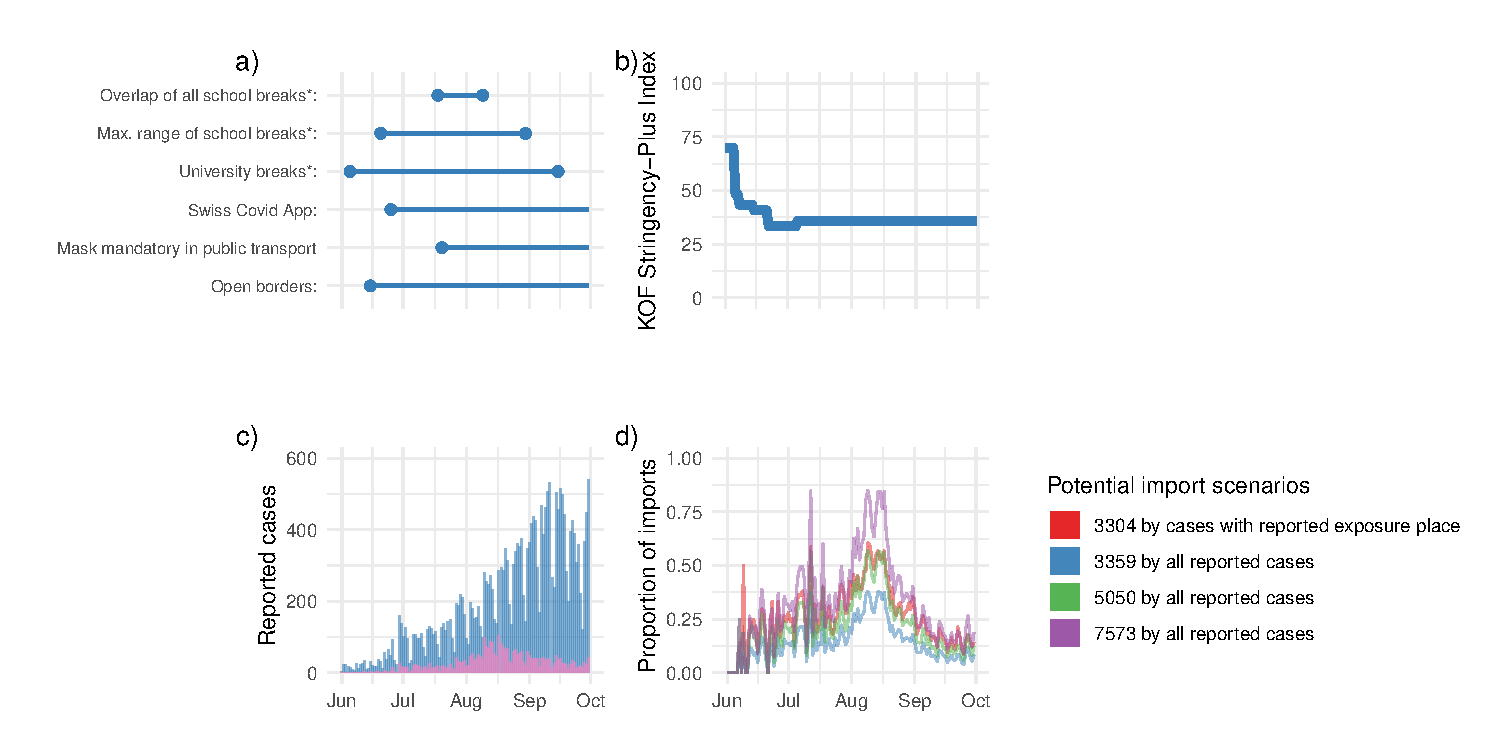
\includegraphics[scale=0.5]{Figure1_2021-04-30.pdf}
\caption{The Swiss SARS-CoV-2 epidemic in summer 2020: 
a) Five major events that might influenced the Swiss epidemic from 1 June to 30 September, 2020. 
b) The KOF stringency plus index records the stringency of COVID-19 policy measures in Switzerland over time.
The values range from 0 (= no measures) to 100 (= full lockdown) (see \href{https://kof.ethz.ch/en/forecasts-and-indicators/indicators/kof-stringency-index.html}{here}. 
c) All reported cases per day (blue) and 3304 cross-border-associated cases (pink).
d) Three cross-border-associated scenarios, i.e., 3,359, 5,050, and 7,573, that were evaluated in the branching process model. 
The SFOPH reported 3,304 cross-border-associated cases and 53\% repoted cases the most likely country of exposure.
$*$Official breaks of universities and schools might vary for different subjects and between different schools and cantons, respectively. 
More details on quarantine measures in Table \ref{t2} and \href{https://www.fedlex.admin.ch/eli/cc/2021/61/de}{here}.}
\label{f1}
\end{figure*}

Beginning of June 2020, Switzerland had an incidence of 0.17 per 100,000 citizens (3 cases) and at the end of September 5.36 (540 cases; Figure \ref{f2}c)
The latter was also the maximum value during the time of interest.
Accordingly, there was an increase during the summer months.
Assuming a constant growth, we estimated an epidemic growth rate of 0.03 (95\%-confidence interval (CI): 0.02-0.03) per day and a $\mathcal{R}_e$ of 1.15 (95\%-CI: 1.14-1.16) for June to September, 2020.
We estimated the 95\%-CI of cumulative incidence of 17,019 to 30,533 cases for 1 June to 30 September, 2020 (23,199 cases were reported by the SFOPH; Figure \ref{f1}a).
For the final incidence the 95\%-CI laid between 93 to 762 cases for the last day (the mean of the reported cases for the last week was 338 cases per day).

\begin{figure*}
\centering
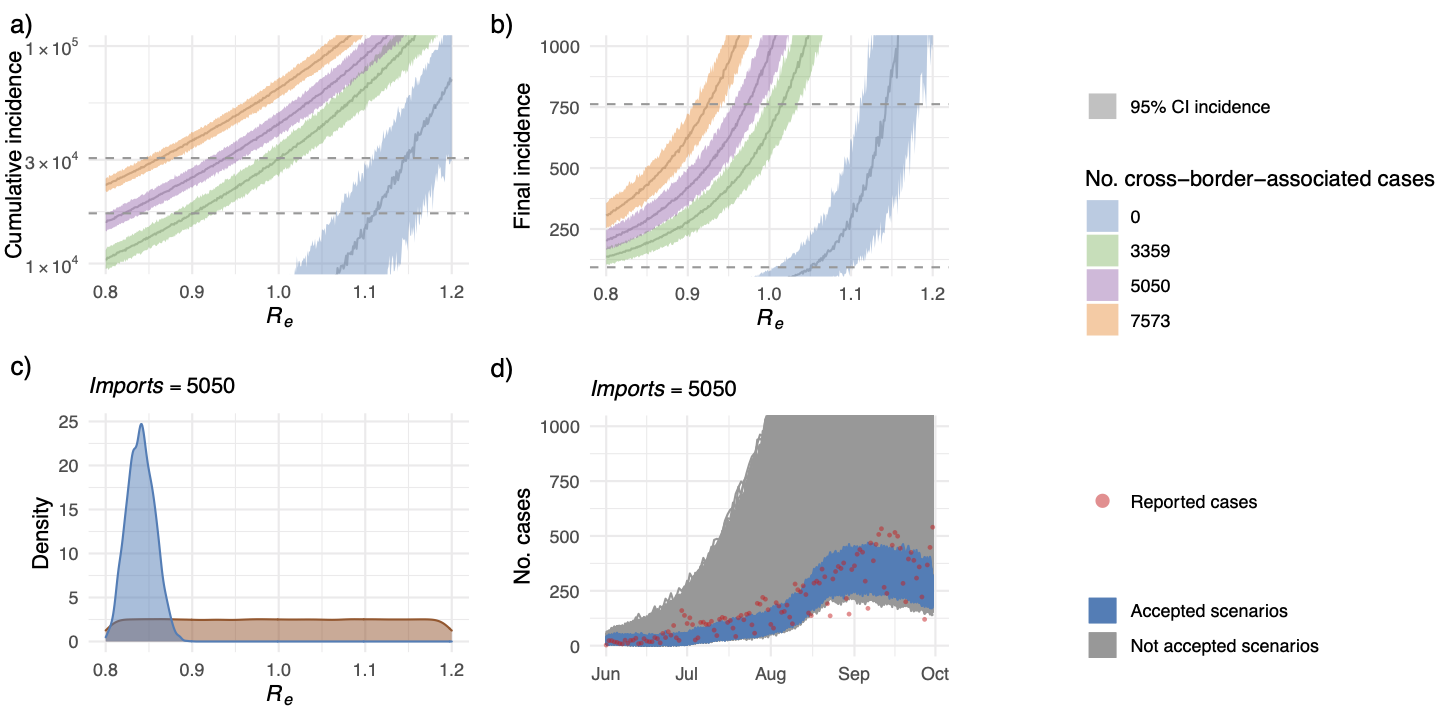
\includegraphics[scale=0.3]{Figure2_2021-04-30.png}
\caption{Impact of cross-border-associated cases on the local epidemic.
a) Curves represent 95\%-CI and median of simulated cumulative incidence with zero, 3,359, 5,050, and 7,573 cross-border-associated cases; expected 95\%-CI of cumulative incidence during $1^{st}$ June to $30^{th}$ September 2020. 
b) Curves represent 95\%-CI and median of simulated final incidence with zero, 3,359, 5,050, and 7,573 cross-border-associated cases; expected 95\%-CI of final incidence on $30^{th}$ September 2020.
c) Prior and posterior distribution of $\mathcal{R}_e$ with 5,050 cross-border-associated cases.
d) Branching trajectories with 5,050 cross-border-associated cases that were within the 95\%-CI of final incidence and cumulative incidence. 
The 95\%-CI of the $\mathcal{R}_e$ of accepted simulations was: 0.84 (95\%-CI: 0.81-0.87).
Abbreviations: CI, credible interval; $R_e$, the reproductive number}

\label{f2}
\end{figure*}

With the branching process model we simulated epidemics using different number of cross-border-associated cases.
Overall, 12,884 of $4*10^5$ (3.22\%) trajectories were within the 95\%-CI of the expected cumulative incidence and final incidence.
The basic model assumed no new introductions which was not the case for the Swiss epidemic and thus, $\mathcal{R}_e$ should be over-estimated.
Accounting for imports requires to re-evaluate the intensity of local transmission (i.e. the value of $\mathcal{R}_e$) to match the observed dynamics of SARS-CoV-2 in summer 2020.
Assuming no introductions, 126 (0.13\%) trajectories were within the 95\%-CI of the expected cumulative incidence and final incidence.
The $\mathcal{R}_e$ was 1.08 (95\%-CI: 1.04-1.11; which was lower not than the $\mathcal{R}_e$ derived from the calculation). (Figure \ref{f1}ab; Supplementary Figure \ref{sf1}).
The basic branching process model was then extended with three scenarios, i.e., 3,359, 5,050, 7,573 introductions of cross-border-associated cases.
In extended models, all cases, i.e., cross-border-associated cases and local cases, were equally likely to transmit SARS-CoV-2.
For 5,050 introductions, corresponding to an extrapolation of 3,304 cross-border-associated cases, 9,197 (9.29\%) trajectories were within the 95\%-CI of the expected cumulative incidence and final incidence (Table \ref{t2}; Figure \ref{f1}).
These 9,291 trajectories had a $\mathcal{R}_e$ of 0.84 (95\%-CI: 0.81-0.87) (Figure \ref{f1}ab; Supplementary Figure \ref{sf1}).
For 3,359 and 7,573 introductions, corresponding to an extrapolation of 3,304 cross-border-associated cases and a multiplication with 2/3 and 1.5, 2,878 (2.88\%) and 589 (0.59\%) trajectories were within the 95\%-CI of the expected cumulative incidence and final incidence (Table \ref{t2}; Figure \ref{f1}).
These 2,878 and 589 trajectories had a $\mathcal{R}_e$ of 0.91 (95\%-CI: 0.88-0.93) and $\mathcal{R}_e$ of 0.80 (95\%-CI: <0.80-0.82) (Figure \ref{f1}ab; Supplementary Figure \ref{sf1}).
To be noted, we were not able to estimate $\mathcal{R}_e$ below 0.80.


\section{Discussion}
The SARS-CoV-2 epidemic in Switzerland grew from a few dozen confirmed cases per day in early June 2020 to several hundred by the end of September 2020. 
Ignoring cross-border-associated cases a constant $\mathcal{R}_e$ was above one for the time of interest. 
In summer 2020, however, around a quarter of cases that had been reported by the SFOPH were cross-border-associated cases.
We also found that different age groups were exposed to the SARS-CoV-2 in different countries abroad.
With our stochastic branching process we showed that the local epidemic had a $\mathcal{R}_e$ below one, i.e. a value below the critical threshold.
At the end of summer 2020, the reported cases stabilised (also in simulations if $\mathcal{R}_e <1$).
Thus, cross-border-associated cases and their local spread was one of the leading forces that led to several hundred cases per day within three months, i.e., by the end of September 2020. 
Consequently, the effect of cross-border-associated cases cannot be ignored in understanding and regulating a local epidemic (during a pandemic).

Our method has several limitations that need to be addressed.
In our stochastic branching process, we did not account for a saisonal effect of the SARS-CoV-2, different restrictions carried out, social contact pattern or age-related mixing patterns.
With our model, we were not interested to simulated single transmission chains.
Our stochastic branching process was calibrated to assess the impact of cross-border-associated cases on an epidemiological, i.e. population-based, level.
Stochastic effects have been showed to play an important role in determining parameters in epidemics.\cite{althaus_ebola_2015,riou_pattern_2020}
The resulted trajectories represent the Swiss epidemic and ignored geographical differences, i.e. cantons.
We found no evidence of relevant geographical differences of cross-border-associated cases (Supplementary Figure \ref{sf3}).
Our approach assumes a constant growth rate over the summer period and ignores immunity, which we consider acceptable during this low prevalence and incidence time:
The SFOPH reported 30,883 cases before 1 June and 23,199 more until 30 September, 2020.
Moreover, growth rates, can be calculated for different intervals, e.g., one week or months and adjusted for different factors, after sensitivity analysis we decided assumes a constant growth rate without any adjustment.
Further, this was more compatible to calculate the overall impact of cross-border-associated cases.

We validated simulated trajectories on well reported data.
However, it is unlikely that all SARS-CoV-2 cases in Switzerland had been tested, but in Switzerland all cases tested have been reported to the FOPH.
Studies reported about a two-fold (or more) underreporting of SARS-CoV-2 infections.\cite{Li_substantial_2020,Wu_substantial_2020}
The degree of under-ascertainment can not be evaluated for the used surveillance data.\textcolor{red}{[true?]}
Moreover, there is a delay of infection to testing and reporting.
We ignored this delay for all cases.
Thus, our simulations reflect the day of testing and reporting and not the start of infection.
During the time of the study, testing was free and mandatory for symptomatic cases, but not for asymptomatic cases.
However, if they had contact with a positive person they were required to do isolate and test themselves. 
The contact tracing was provided either by infectees themselves, through authorities or the Swiss Covid app (launched on 15 June 2020).\cite{salath_early_2020}

As our study period covered only summer seasonality should have no influence.
However, people were more active during summer than during winter and likely more optimistic about the pandemic (mostly at the end of summer 2020), which likely resulted in more social contacts than before.
Tracking contact patterns, i.e., behaviour, can give a more rapid assessment of the impact of physical distancing measures than routine epidemiological surveillance.\cite{jarvis_quantifying_2020}
Unfortunately, social contact pattern or age-related mixing patterns are missing for this time in Switzerland.
Such information of a representative study population, like established by the Co-Mix study, are needed to better understand the social dynamics.\cite{coletti_comix_2020}
This highlights the importance of implementing and following up the Co-Mix study and other studies.
Our study indicated that to understand the spread of SARS-CoV-2 age-related mixing patterns need to be known.
However, close contact alone is not responsible for SARS-CoV-2 transmission.
Some transmission cluster were linked to indoor crowded spaces which underlines the possibility of aerosol (and droplet) transmission.\cite{tang_aerosol_2020}
Our study design was appropriate for our research question.
Nevertheless, there is a need of analyses that include several more variables, such as age-contact pattern, saisonal- or climate changes.
These will help to more precisely forecast future outbreaks and pandemics.

Our results are important to derive travel strategies, including mandatory quarantine and test strategies for the coming summer 2021.
Also in other countries, travel had a strong impact on the local epidemic.\cite{russell_effect_2021,hodcroft_emergence_2020}
It is likely that (global) herd immunity will not be achieved in the summer 2021, so existing measures such as testing and physical distancing remain important to keep incidence low.
In addition, there is still uncertainty about asymptomatic cases.\cite{nogrady_what_2020}
Studies found the proportion of asymptomatic cases to be 17\% (or 20\%) and 1/4 less transmissible.\cite{byambasuren_estimating_2020,buitrago-garcia_occurrence_2020,bi_household_2020}
It could be an option to test all people that cross borders and give them the option of reduced quarantine for negative cases.\cite{ashcroft_quantifying_2021}
In the beginning of July 2020, only five countries from 21 countries with at least a dozen cross-border-associated cases were on the list to do mandatory quarantine if returned.
A handful of countries of these 21 had not been on the list during summer.
Mandatory quarantine and testing might reduce the willingness to travel as the effort and awareness of the SARS-CoV-2 pandemic will remain.
Thus, travel mobility might be reduced, and cross-border-associated cases and their local spreading might be minimised through testing and mandatory quarantine.



Switzerland is a relatively small country with few million citizens, but due to its location (and its wealth) there is a high potential for travel which might have a huge impact on the epidemic.
Quantifying the role of imports on the national dynamics of SARS-CoV-2 epidemics requires further investigation. 
In Switzerland, cross-border-associated cases have had a considerable impact on the national dynamics and could explain the growth of the SARS-CoV-2 epidemic during summer 2020. 
Our results underline the importance of improved surveillance for international travellers in order to better control the spread of SARS-CoV-2.


\section{Acknowledgement}
We thank the FOPH.  Calculations were performed on UBELIX (http://www.id.unibe.ch/hpc), the HPC cluster at the University of Bern.

\section{Author contributions}
MLR, EBH, JR, NAR, and CLR conceived the study and contributed to the analysis of the results. 
MLR performed the analysis and wrote the first draft of the manuscript. 
NH gave important inputs for the analysis and interpretation. 
All authors read and approved the final manuscript.

\section{Funding}
European Union’s Horizon 2020 research and innovation programme - project EpiPose (No 101003688). Swiss National Science Foundation (grant 196046)

\section{Reference}
\bibliography{../manuscript/su2020_cov2.bib}
\bibliographystyle{vancouver}

\end{multicols}

\clearpage
\begin{suppfigure}[h]
\centering
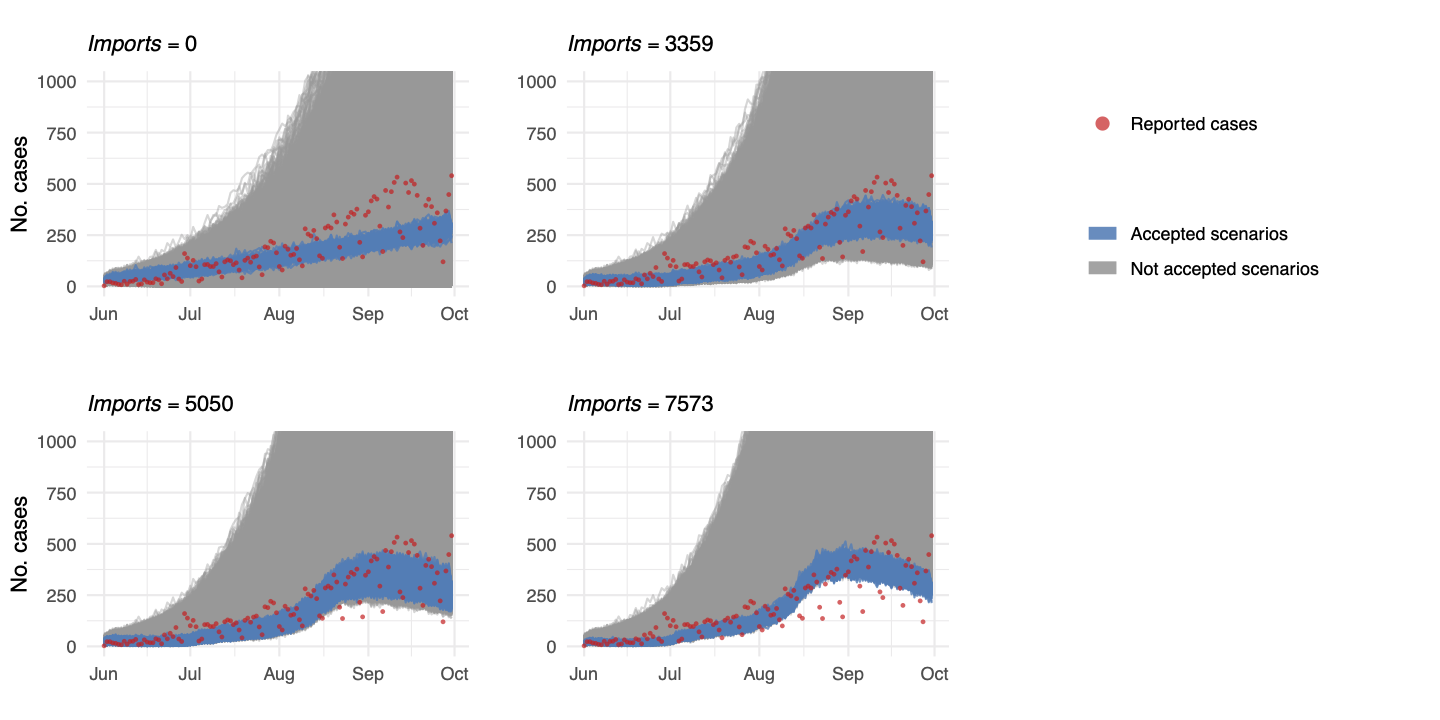
\includegraphics[scale=0.4]{SF1_2021-04-30.png}
\caption{Impact of cross-border-associated cases on the local epidemic: 
Branching trajectories with 0, 3,359, 5,050, and 7,573, cross-border-associated cases that were within the 95\%-CI of final incidence and cumulative incidence. 
Abbreviations: CI, credible interval; $R_e$, the reproductive number}
\label{sf1}
\end{suppfigure}


\clearpage
\begin{suppfigure}[h]
\centering
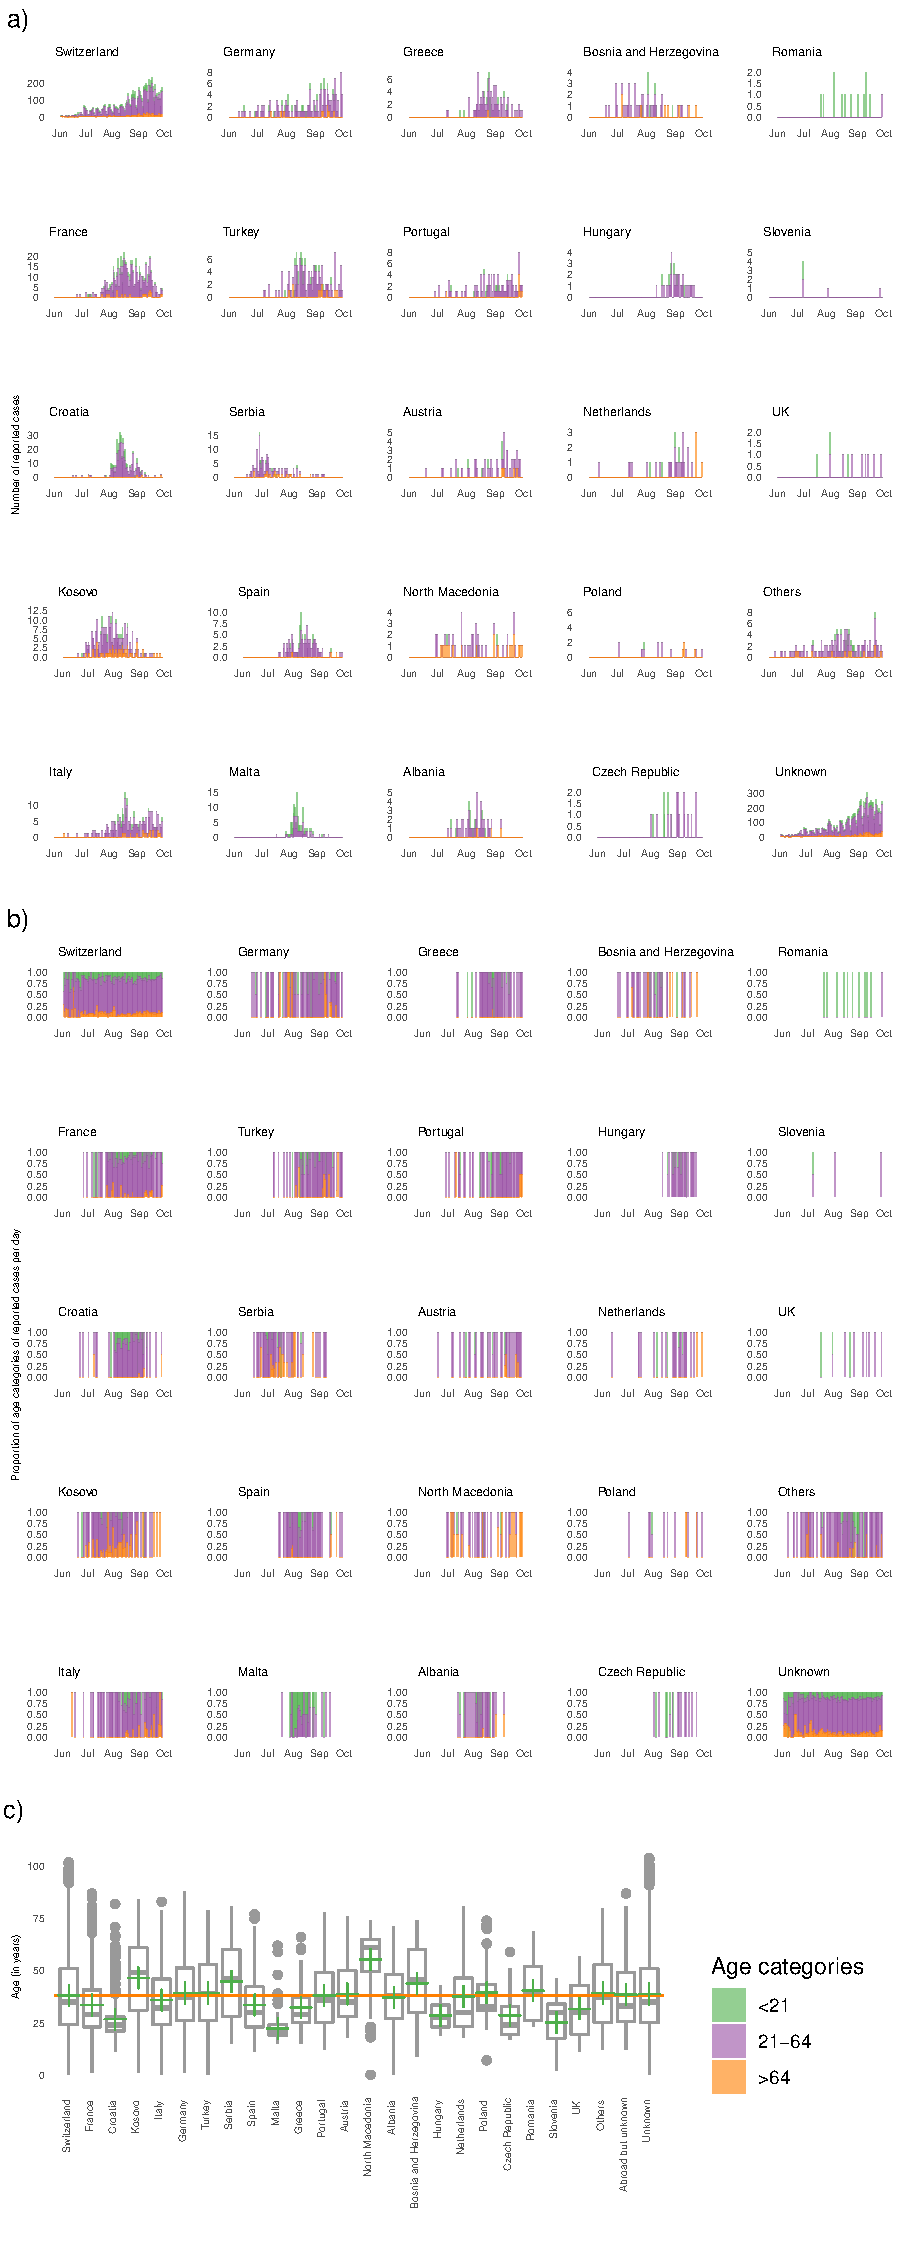
\includegraphics[scale=0.6]{SF2_2021-04-30.pdf}
\caption{Reported cases and the most likely country of exposure.
a) number of reported cases and fraction of different age groups.
b) proportion of all cases and proportion of different age groups.
c) Age distribution for reported cases according to the most likely country of exposure.
+ represents the mean of the age in the corresponding group, the horizontal line is the mean of the age of all cases that were exposed only in Switzerland.}
\label{sf2}
\end{suppfigure}


\clearpage
\begin{suppfigure}[h]
\centering
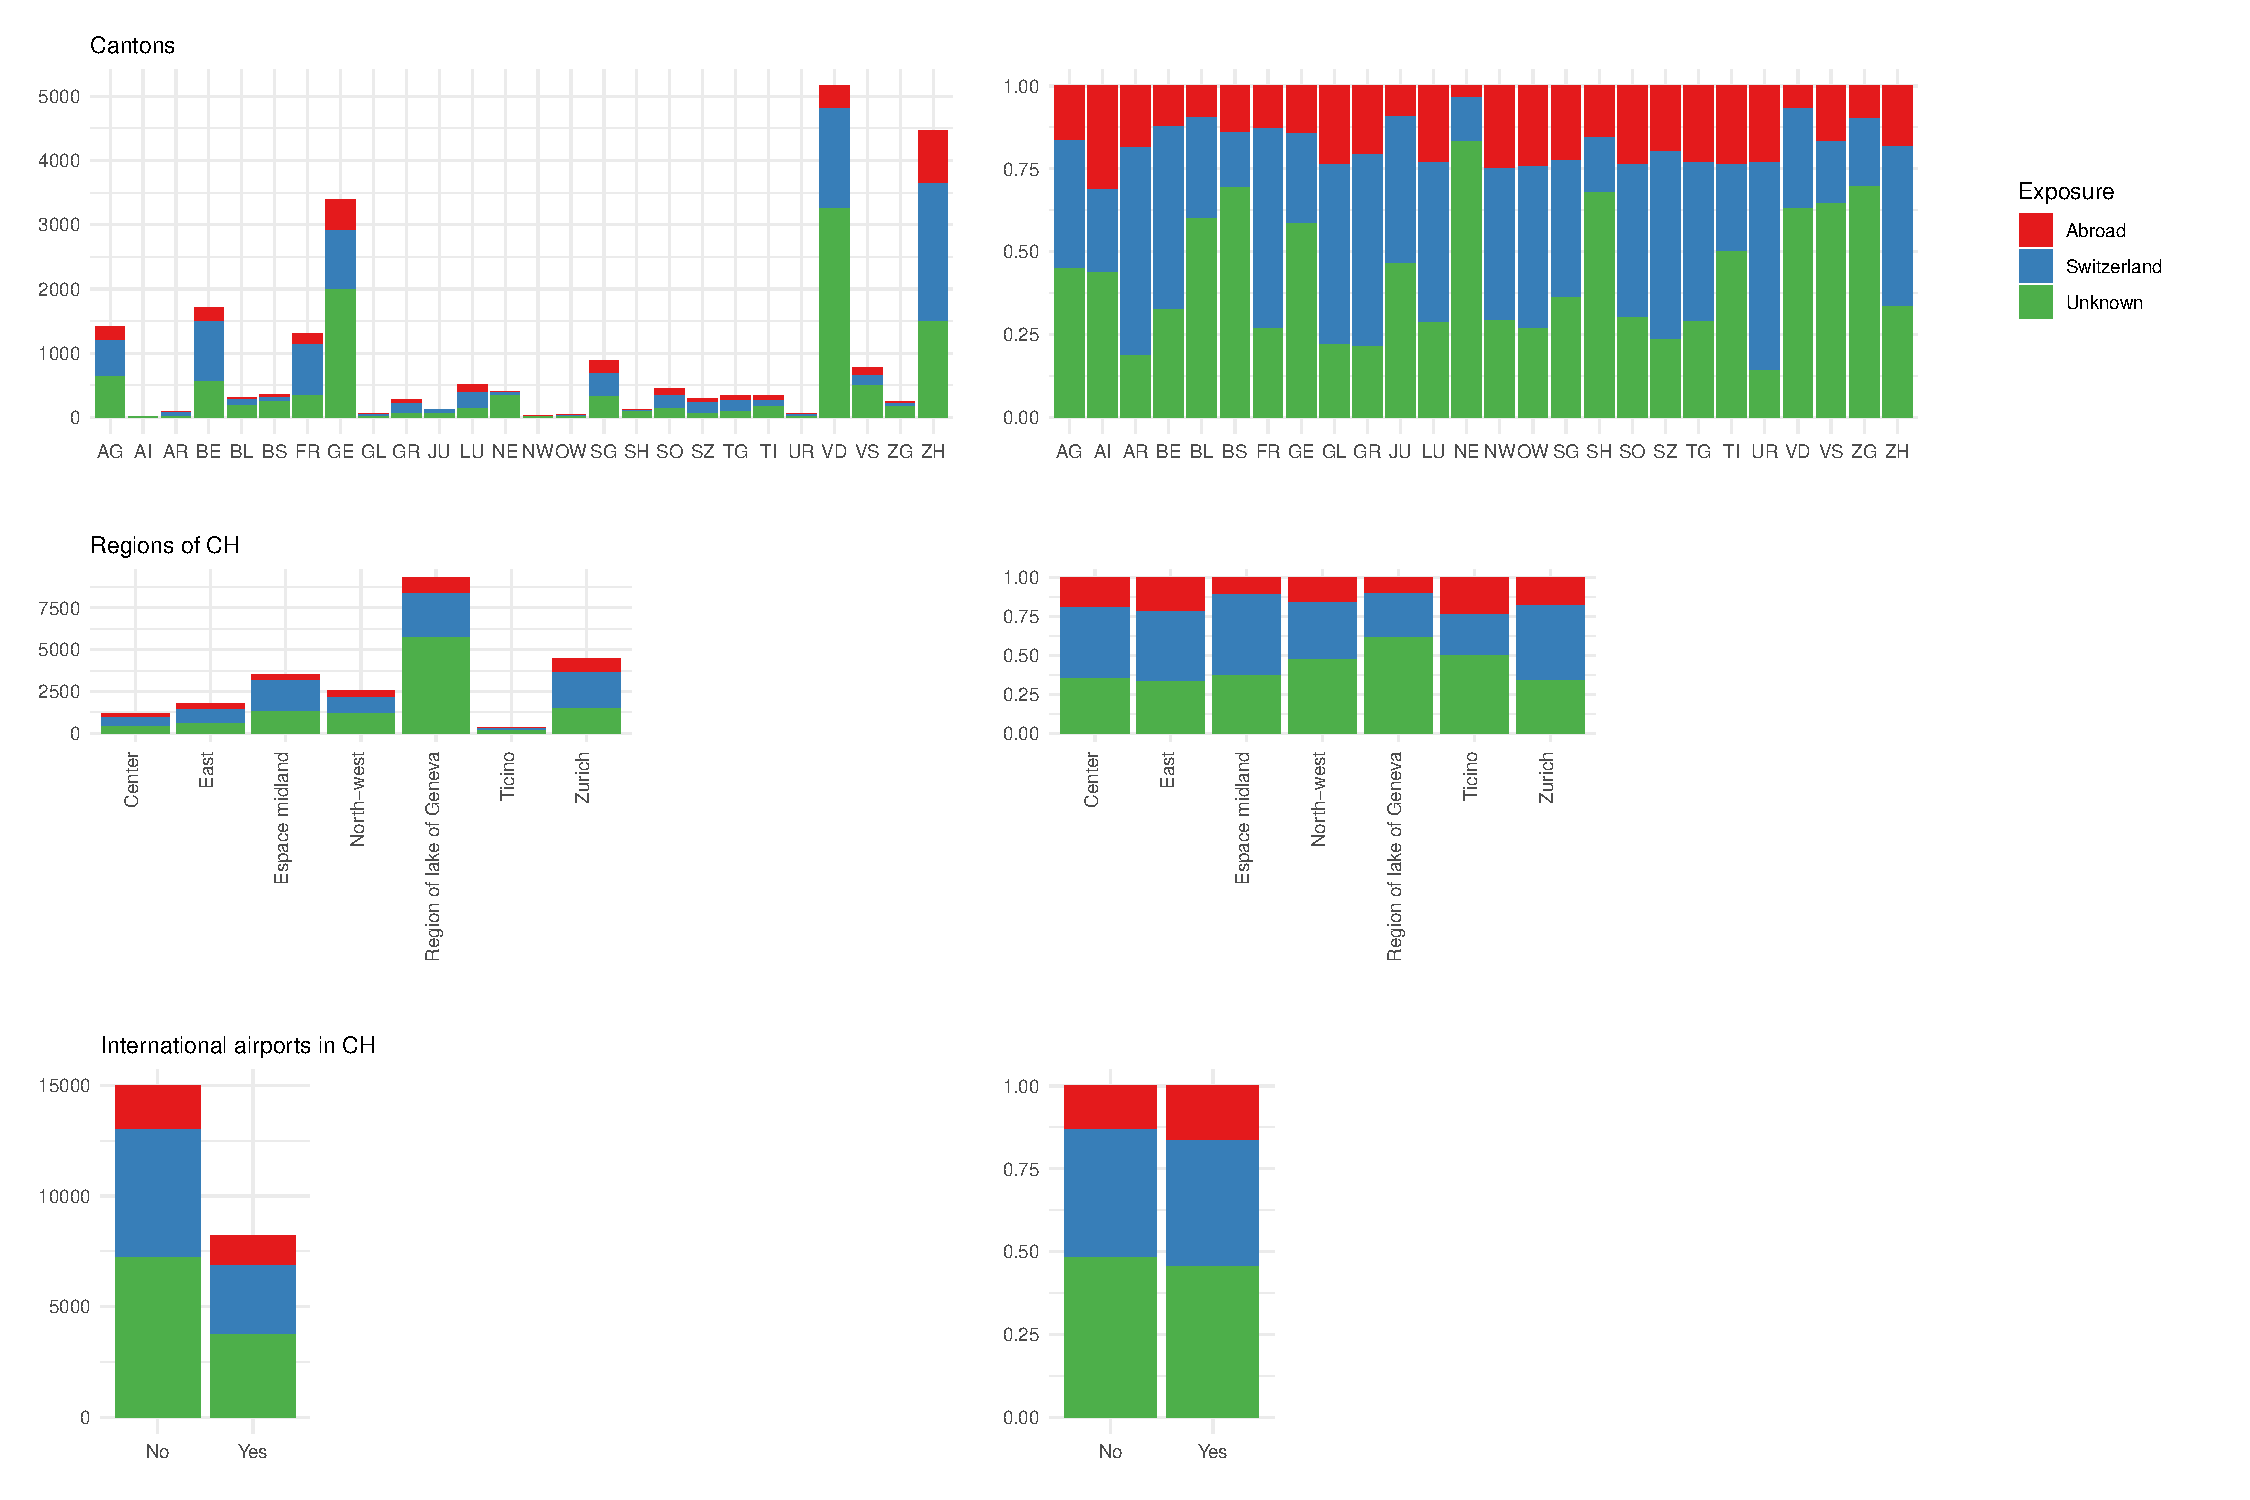
\includegraphics[scale=0.4]{SF3_2021-04-30.pdf}
\caption{Place and region of residency regarding reported exposure places}
\label{sf3}
\end{suppfigure}


\end{document}